\section{Specific Latent Heat of Fusion in Ice}
CPACs 1 and 4
\hfill
\nth{21} January 2020

\subsection{Abstract}
In this experiment the specific latent heat of fusion in ice was experimentally found using two differant methods.

\subsubsection{Equiptment}
\begin{itemize}
\item Large plastic funnel
\item Beakers
\item Low-voltage heater
\item Clamp and stand
\item Mercury thermometer
\item Low-voltage power supply
\item Ammeter
\item Voltmeter
\item Stopwatch
\item Top-pan balance
\item Switch
\item Variable resistor
\item Ice cubes
\item Stopwatch
\end{itemize}

\subsubsection{Method}
\begin{enumerate}
\item Position a funnel filled with ice above a plastic beaker sitting on a top-pan balance.
\item Clamp a low-voltage electrical heater maximising the surface contact between the ice and the heater.
\item Connect the heater to the circuit and record the current and voltage.
\item Once the rate of melting of the ice is steady, zero the top-pan balance and start a stopwatch.
\end{enumerate}

\subsubsection{Diagram}
\begin{figure}
    \centering
    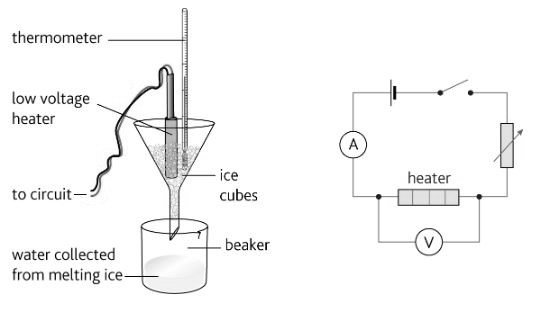
\includegraphics[width=8cm]{i_t2_b}
    \caption{Diagram for Exp. B}
\end{figure}

\subsubsection{Results}
The following results where recorded:
\begin{center}
    \begin{tabular}{ |c|c| } 
        \hline
        Time Period & 600s \\ \hline
        Mass of Water & 44.99g\\ \hline
        Current & 2.55A \\ \hline
        Voltage & 8.06V \\
        \hline
        \end{tabular}
\end{center}

\subsubsection{Calculation}
Electrical energy supplied to heater is:
\begin{equation*}
    E = I \cdot V \cdot t \\
    E = 2.55 \cdot 8.06 \cdot 600 = 12331.8J\\
\end{equation*}

The specific latent heat of fusion is defined to be:
\begin{equation*}
    L = \frac{Q}{m}
\end{equation*}

From the data in our experiment we obtain a specific latent heat of fusion of:
\begin{equation*}
    L = \frac{12331.8}{0.004499} = 274100 J {kg}^{-1}
\end{equation*}

\subsubsection{Evaluation}
The specific latent heat of fusion for water is 334,000 $J {kg}^{-1}$

As a result the percentage difference is:
\begin{equation*}
    \frac{334000-274100}{334000} = 17.9 \%
\end{equation*}

As all data was recorded electronically there is negligable percentage error in the measurements.

\subsubsection{Analyis}
